% !TEX root = tnnls_relation_gait.tex

\ifx\allfiles\undefined
    % !TEX root = tnnls_relation_gait.tex

%% bare_jrnl.tex
%% V1.4b
%% 2015/08/26
%% by Michael Shell
%% see http://www.michaelshell.org/
%% for current contact information.
%%
%% This is a skeleton file demonstrating the use of IEEEtran.cls
%% (requires IEEEtran.cls version 1.8b or later) with an IEEE
%% journal paper.
%%
%% Support sites:
%% http://www.michaelshell.org/tex/ieeetran/
%% http://www.ctan.org/pkg/ieeetran
%% and
%% http://www.ieee.org/

%%*************************************************************************
%% Legal Notice:
%% This code is offered as-is without any warranty either expressed or
%% implied; without even the implied warranty of MERCHANTABILITY or
%% FITNESS FOR A PARTICULAR PURPOSE!
%% User assumes all risk.
%% In no event shall the IEEE or any contributor to this code be liable for
%% any damages or losses, including, but not limited to, incidental,
%% consequential, or any other damages, resulting from the use or misuse
%% of any information contained here.
%%
%% All comments are the opinions of their respective authors and are not
%% necessarily endorsed by the IEEE.
%%
%% This work is distributed under the LaTeX Project Public License (LPPL)
%% ( http://www.latex-project.org/ ) version 1.3, and may be freely used,
%% distributed and modified. A copy of the LPPL, version 1.3, is included
%% in the base LaTeX documentation of all distributions of LaTeX released
%% 2003/12/01 or later.
%% Retain all contribution notices and credits.
%% ** Modified files should be clearly indicated as such, including  **
%% ** renaming them and changing author support contact information. **
%%*************************************************************************


% *** Authors should verify (and, if needed, correct) their LaTeX system  ***
% *** with the testflow diagnostic prior to trusting their LaTeX platform ***
% *** with production work. The IEEE's font choices and paper sizes can   ***
% *** trigger bugs that do not appear when using other class files.       ***                          ***
% The testflow support page is at:
% http://www.michaelshell.org/tex/testflow/

\documentclass[journal]{IEEEtran}
%
% If IEEEtran.cls has not been installed into the LaTeX system files,
% manually specify the path to it like:
% \documentclass[journal]{../sty/IEEEtran}

% Some very useful LaTeX packages include:
% (uncomment the ones you want to load)

% *** MISC UTILITY PACKAGES ***
%
%\usepackage{ifpdf}
% Heiko Oberdiek's ifpdf.sty is very useful if you need conditional
% compilation based on whether the output is pdf or dvi.
% usage:
% \ifpdf
%   % pdf code
% \else
%   % dvi code
% \fi
% The latest version of ifpdf.sty can be obtained from:
% http://www.ctan.org/pkg/ifpdf
% Also, note that IEEEtran.cls V1.7 and later provides a builtin
% \ifCLASSINFOpdf conditional that works the same way.
% When switching from latex to pdflatex and vice-versa, the compiler may
% have to be run twice to clear warning/error messages.

% *** CITATION PACKAGES ***

\usepackage{tabularx}
\usepackage{longtable}
\usepackage{threeparttable}
\usepackage{cite}

% cite.sty was written by Donald Arseneau
% V1.6 and later of IEEEtran pre-defines the format of the cite.sty package
% \cite{} output to follow that of the IEEE. Loading the cite package will
% result in citation numbers being automatically sorted and properly
% "compressed/ranged". e.g., [1], [9], [2], [7], [5], [6] without using
% cite.sty will become [1], [2], [5]--[7], [9] using cite.sty. cite.sty's
% \cite will automatically add leading space, if needed. Use cite.sty's
% noadjust option (cite.sty V3.8 and later) if you want to turn this off
% such as if a citation ever needs to be enclosed in parenthesis.
% cite.sty is already installed on most LaTeX systems. Be sure and use
% version 5.0 (2009-03-20) and later if using hyperref.sty.
% The latest version can be obtained at:
% http://www.ctan.org/pkg/cite
% The documentation is contained in the cite.sty file itself.

% *** GRAPHICS RELATED PACKAGES ***
%
\usepackage[pdftex]{graphicx}
\usepackage{rotating}
\ifCLASSINFOpdf
  % \usepackage[pdftex]{graphicx}
  % declare the path(s) where your graphic files are
  % \graphicspath{{../pdf/}{../jpeg/}}
  % and their extensions so you won't have to specify these with
  % every instance of \includegraphics
  % \DeclareGraphicsExtensions{.pdf,.jpeg,.png}
\else
  % or other class option (dvipsone, dvipdf, if not using dvips). graphicx
  % will default to the driver specified in the system graphics.cfg if no
  % driver is specified.
  % \usepackage[dvips]{graphicx}
  % declare the path(s) where your graphic files are
  % \graphicspath{{../eps/}}
  % and their extensions so you won't have to specify these with
  % every instance of \includegraphics
  % \DeclareGraphicsExtensions{.eps}
\fi
% graphicx was written by David Carlisle and Sebastian Rahtz. It is
% required if you want graphics, photos, etc. graphicx.sty is already
% installed on most LaTeX systems. The latest version and documentation
% can be obtained at:
% http://www.ctan.org/pkg/graphicx
% Another good source of documentation is "Using Imported Graphics in
% LaTeX2e" by Keith Reckdahl which can be found at:
% http://www.ctan.org/pkg/epslatex
%
% latex, and pdflatex in dvi mode, support graphics in encapsulated
% postscript (.eps) format. pdflatex in pdf mode supports graphics
% in .pdf, .jpeg, .png and .mps (metapost) formats. Users should ensure
% that all non-photo figures use a vector format (.eps, .pdf, .mps) and
% not a bitmapped formats (.jpeg, .png). The IEEE frowns on bitmapped formats
% which can result in "jaggedy"/blurry rendering of lines and letters as
% well as large increases in file sizes.
%
% You can find documentation about the pdfTeX application at:
% http://www.tug.org/applications/pdftex

% *** MATH PACKAGES ***
%
\usepackage{amsmath}
% A popular package from the American Mathematical Society that provides
% many useful and powerful commands for dealing with mathematics.
%
% Note that the amsmath package sets \interdisplaylinepenalty to 10000
% thus preventing page breaks from occurring within multiline equations. Use:
%\interdisplaylinepenalty=2500
% after loading amsmath to restore such page breaks as IEEEtran.cls normally
% does. amsmath.sty is already installed on most LaTeX systems. The latest
% version and documentation can be obtained at:
% http://www.ctan.org/pkg/amsmath

% *** SPECIALIZED LIST PACKAGES ***
%
\usepackage{algorithmic}
% algorithmic.sty was written by Peter Williams and Rogerio Brito.
% This package provides an algorithmic environment fo describing algorithms.
% You can use the algorithmic environment in-text or within a figure
% environment to provide for a floating algorithm. Do NOT use the algorithm
% floating environment provided by algorithm.sty (by the same authors) or
% algorithm2e.sty (by Christophe Fiorio) as the IEEE does not use dedicated
% algorithm float types and packages that provide these will not provide
% correct IEEE style captions. The latest version and documentation of
% algorithmic.sty can be obtained at:
% http://www.ctan.org/pkg/algorithms
% Also of interest may be the (relatively newer and more customizable)
% algorithmicx.sty package by Szasz Janos:
% http://www.ctan.org/pkg/algorithmicx

% *** ALIGNMENT PACKAGES ***
%
\usepackage{array}
% Frank Mittelbach's and David Carlisle's array.sty patches and improves
% the standard LaTeX2e array and tabular environments to provide better
% appearance and additional user controls. As the default LaTeX2e table
% generation code is lacking to the point of almost being broken with
% respect to the quality of the end results, all users are strongly
% advised to use an enhanced (at the very least that provided by array.sty)
% set of table tools. array.sty is already installed on most systems. The
% latest version and documentation can be obtained at:
% http://www.ctan.org/pkg/array

% IEEEtran contains the IEEEeqnarray family of commands that can be used to
% generate multiline equations as well as matrices, tables, etc., of high
% quality.

% *** SUBFIGURE PACKAGES ***
\usepackage[caption=false,font=footnotesize]{subfig}
%\ifCLASSOPTIONcompsoc
%  \usepackage[caption=false,font=normalsize,labelfont=sf,textfont=sf]{subfig}
%\else
%  \usepackage[caption=false,font=footnotesize]{subfig}
%\fi
% subfig.sty, written by Steven Douglas Cochran, is the modern replacement
% for subfigure.sty, the latter of which is no longer maintained and is
% incompatible with some LaTeX packages including fixltx2e. However,
% subfig.sty requires and automatically loads Axel Sommerfeldt's caption.sty
% which will override IEEEtran.cls' handling of captions and this will result
% in non-IEEE style figure/table captions. To prevent this problem, be sure
% and invoke subfig.sty's "caption=false" package option (available since
% subfig.sty version 1.3, 2005/06/28) as this is will preserve IEEEtran.cls
% handling of captions.
% Note that the Computer Society format requires a larger sans serif font
% than the serif footnote size font used in traditional IEEE formatting
% and thus the need to invoke different subfig.sty package options depending
% on whether compsoc mode has been enabled.
%
% The latest version and documentation of subfig.sty can be obtained at:
% http://www.ctan.org/pkg/subfig

% *** FLOAT PACKAGES ***
%
%\usepackage{fixltx2e}
% fixltx2e, the successor to the earlier fix2col.sty, was written by
% Frank Mittelbach and David Carlisle. This package corrects a few problems
% in the LaTeX2e kernel, the most notable of which is that in current
% LaTeX2e releases, the ordering of single and double column floats is not
% guaranteed to be preserved. Thus, an unpatched LaTeX2e can allow a
% single column figure to be placed prior to an earlier double column
% figure.
% Be aware that LaTeX2e kernels dated 2015 and later have fixltx2e.sty's
% corrections already built into the system in which case a warning will
% be issued if an attempt is made to load fixltx2e.sty as it is no longer
% needed.
% The latest version and documentation can be found at:
% http://www.ctan.org/pkg/fixltx2e

%\usepackage{stfloats}
% stfloats.sty was written by Sigitas Tolusis. This package gives LaTeX2e
% the ability to do double column floats at the bottom of the page as well
% as the top. (e.g., "\begin{figure*}[!b]" is not normally possible in
% LaTeX2e). It also provides a command:
%\fnbelowfloat
% to enable the placement of footnotes below bottom floats (the standard
% LaTeX2e kernel puts them above bottom floats). This is an invasive package
% which rewrites many portions of the LaTeX2e float routines. It may not work
% with other packages that modify the LaTeX2e float routines. The latest
% version and documentation can be obtained at:
% http://www.ctan.org/pkg/stfloats
% Do not use the stfloats baselinefloat ability as the IEEE does not allow
% \baselineskip to stretch. Authors submitting work to the IEEE should note
% that the IEEE rarely uses double column equations and that authors should try
% to avoid such use. Do not be tempted to use the cuted.sty or midfloat.sty
% packages (also by Sigitas Tolusis) as the IEEE does not format its papers in
% such ways.
% Do not attempt to use stfloats with fixltx2e as they are incompatible.
% Instead, use Morten Hogholm'a dblfloatfix which combines the features
% of both fixltx2e and stfloats:
%
% \usepackage{dblfloatfix}
% The latest version can be found at:
% http://www.ctan.org/pkg/dblfloatfix

%\ifCLASSOPTIONcaptionsoff
%  \usepackage[nomarkers]{endfloat}
% \let\MYoriglatexcaption\caption
% \renewcommand{\caption}[2][\relax]{\MYoriglatexcaption[#2]{#2}}
%\fi
% endfloat.sty was written by James Darrell McCauley, Jeff Goldberg and
% Axel Sommerfeldt. This package may be useful when used in conjunction with
% IEEEtran.cls'  captionsoff option. Some IEEE journals/societies require that
% submissions have lists of figures/tables at the end of the paper and that
% figures/tables without any captions are placed on a page by themselves at
% the end of the document. If needed, the draftcls IEEEtran class option or
% \CLASSINPUTbaselinestretch interface can be used to increase the line
% spacing as well. Be sure and use the nomarkers option of endfloat to
% prevent endfloat from "marking" where the figures would have been placed
% in the text. The two hack lines of code above are a slight modification of
% that suggested by in the endfloat docs (section 8.4.1) to ensure that
% the full captions always appear in the list of figures/tables - even if
% the user used the short optional argument of \caption[]{}.
% IEEE papers do not typically make use of \caption[]'s optional argument,
% so this should not be an issue. A similar trick can be used to disable
% captions of packages such as subfig.sty that lack options to turn off
% the subcaptions:
% For subfig.sty:
% \let\MYorigsubfloat\subfloat
% \renewcommand{\subfloat}[2][\relax]{\MYorigsubfloat[]{#2}}
% However, the above trick will not work if both optional arguments of
% the \subfloat command are used. Furthermore, there needs to be a
% description of each subfigure *somewhere* and endfloat does not add
% subfigure captions to its list of figures. Thus, the best approach is to
% avoid the use of subfigure captions (many IEEE journals avoid them anyway)
% and instead reference/explain all the subfigures within the main caption.
% The latest version of endfloat.sty and its documentation can obtained at:
% http://www.ctan.org/pkg/endfloat
%
% The IEEEtran \ifCLASSOPTIONcaptionsoff conditional can also be used
% later in the document, say, to conditionally put the References on a
% page by themselves.

% *** PDF, URL AND HYPERLINK PACKAGES ***
%
\usepackage{url}
% url.sty was written by Donald Arseneau. It provides better support for
% handling and breaking URLs. url.sty is already installed on most LaTeX
% systems. The latest version and documentation can be obtained at:
% http://www.ctan.org/pkg/url
% Basically, \url{my_url_here}.

% *** Do not adjust lengths that control margins, column widths, etc. ***
% *** Do not use packages that alter fonts (such as pslatex).         ***
% There should be no need to do such things with IEEEtran.cls V1.6 and later.
% (Unless specifically asked to do so by the journal or conference you plan
% to submit to, of course. )

% correct bad hyphenation here
% \hyphenation{op-tical net-works semi-conduc-tor}
\usepackage{enumerate}
\usepackage{multirow}
\usepackage{color}
\usepackage{threeparttable}
\usepackage{booktabs}
\newcommand{\minus}{\scalebox{0.75}[1.0]{$-$}}
\newcommand{\bftab}[1]{{\fontseries{b}\selectfont#1}}
\newcommand{\tabincell}[2]{\begin{tabular}{@{}#1@{}}#2\end{tabular}}
\newcommand{\etal}{\textit{et al}.}
\newcommand{\ie}{\textit{i.e.}}
\newcommand{\eg}{\textit{e.g.}}
\newcommand{\wrt}{\textit{w.r.t.}}
\newcommand{\vs}{\textit{vs.}}


\begin{document}
%
% paper title
% Titles are generally capitalized except for words such as a, an, and, as,
% at, but, by, for, in, nor, of, on, or, the, to and up, which are usually
% not capitalized unless they are the first or last word of the title.
% Linebreaks \\ can be used within to get better formatting as desired.
% Do not put math or special symbols in the title.
%\title{The Application and Research of Multi-modal Data in Auxiliary Diagnosis of Depression: A Survey
%}
\title{ Auxiliary Diagnosis of Depression Based on Multi-modal Data: A Survey
}
%%
%%
%% author names and IEEE memberships
%% note positions of commas and nonbreaking spaces ( ~ ) LaTeX will not break
%% a structure at a ~ so this keeps an author's name from being broken across
%% two lines.
%% use \thanks{} to gain access to the first footnote area
%% a separate \thanks must be used for each paragraph as LaTeX2e's \thanks
%% was not built to handle multiple paragraphs
%%
%
%\author{Saihui~Hou,
%	Xu~Liu,
%	Chunshui~Cao,
%	and~Yongzhen~Huang$^*$% <-this % stops a space
%	\thanks{$^*$ indicates the corresponding author.}% <-this % stops a space
%    \thanks{Saihui Hou and Yongzhen Huang is with School of Artificial Intelligence, Beijing Normal University, Beijing 100875, China. (Email: housaihui@bnu.edu.cn, huangyongzhen@bnu.edu.cn)}
%	\thanks{Xu Liu and Chunshui Cao are with Watrix Technology Limited Co. Ltd, Beijing 100088, China. (Email: xu.liu@watrix.ai, chunshuicao@watrix.ai)}
%    \thanks{This work is partially supported by the Fundamental Research Funds for the Central Universities.}
%    % \thanks{E-mail: housaihui@bnu.edu.cn, xu.liu@watrix.ai, chunshuicao@watrix.ai, huangyongzhen@bnu.edu.cn}
%	% \thanks{Manuscript received April 19, 2005; revised August 26, 2015.}
%}
%
%% note the % following the last \IEEEmembership and also \thanks -
%% these prevent an unwanted space from occurring between the last author name
%% and the end of the author line. i.e., if you had this:
%%
%% \author{....lastname \thanks{...} \thanks{...} }
%%                     ^------------^------------^----Do not want these spaces!
%%
%% a space would be appended to the last name and could cause every name on that
%% line to be shifted left slightly. This is one of those "LaTeX things". For
%% instance, "\textbf{A} \textbf{B}" will typeset as "A B" not "AB". To get
%% "AB" then you have to do: "\textbf{A}\textbf{B}"
%% \thanks is no different in this regard, so shield the last } of each \thanks
%% that ends a line with a % and do not let a space in before the next \thanks.
%% Spaces after \IEEEmembership other than the last one are OK (and needed) as
%% you are supposed to have spaces between the names. For what it is worth,
%% this is a minor point as most people would not even notice if the said evil
%% space somehow managed to creep in.
%
%% The paper headers
%\markboth{IEEE Transactions on Neural Networks and Learning Systems}%
%{Saihui Hou \MakeLowercase{\textit{et al.}}: GQAN: Towards the Interpretability of Silhouette-based Gait Recognition}
%% The only time the second header will appear is for the odd numbered pages
%% after the title page when using the twoside option.
%%
%% *** Note that you probably will NOT want to include the author's ***
%% *** name in the headers of peer review papers.                   ***
%% You can use \ifCLASSOPTIONpeerreview for conditional compilation here if
%% you desire.
%
%% If you want to put a publisher's ID mark on the page you can do it like
%% this:
%%\IEEEpubid{0000--0000/00\$00.00~\copyright~2015 IEEE}
%% Remember, if you use this you must call \IEEEpubidadjcol in the second
%% column for its text to clear the IEEEpubid mark.
%
%% use for special paper notices
%%\IEEEspecialpapernotice{(Invited Paper)}
%
%% make the title area
\maketitle

\fi

%\section{Depression Recognition}
%\section{Depression recognition method based on gait}
\subsection{Gait}
%%%%%%%%%%%%%%%%%%%%%%%%%%%%%%%%%%%%%%%%%%%%%%%%%%%%%%%
Human gait, as a daily movement, occurs in parallel with the development of higher brain structures and functions (prefrontal cortex, basal ganglia and cerebellum) and reflects the integrity of the higher brain systems\cite{sheridan2007role}, thus it is a good indicator of mental status.
Compared to traditional mental illness detection biometrics, such as facial expression, speech and physiological parameters, gait is remotely observable, more difficult to imitate, and requires less cooperation from the subject. These advantages make gait a promising source for depression recognition.

Furthermore, researchers have also studied the gait characteristics of depression patients through motion analysis.
Specifically, Lemake et al. [29] calculated the spatiotemporal gait parameters of patients with major depression disorder and found that the patients show significant reductions in stride length, cycle time, and lower limb support.
Moreover, by using the motion capture system with video cameras, Michalak\cite{michalak2009embodiment} found reduced walking velocity, arm swing, vertical body movement, increased body sway and more slumped posture in patients.
Slumped posture is often observed in depressive individuals during sitting, standing and walking.
Thanks to the development of consumer-grade depth cameras (e.g., Kinect, the data collection
scheme is shown in Fig~\ref{kinect}), human body dynamics can be traced accurately in a three dimensional manner without the assistance of the attached markers or the requirement of a specifically designed environment. The recorded depth and skeleton data have been widely and successfully used in depression recognition.
Therefore, in the current studies of depression recognition, the main work is to learn gait features from the skeleton coordinates recorded by Kinect related with depression and explore feature set for better performance.
In the meantime, traditional machine learning algorithms are employed to classify such as SVM, KNN , RF, etc. However, deep learning methods have made breakthroughs in the research fields of both Computer Vision (CV). Therefore, many studies are shifting from the traditional hand crafted gait features to the framework based on deep learning for gait depression recognition.

\begin{figure}
\centering
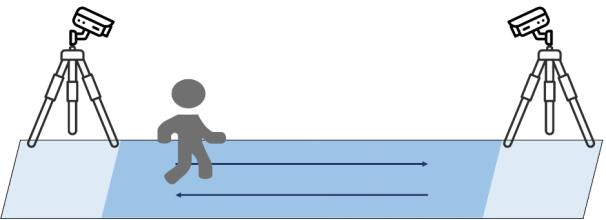
\includegraphics[height=3cm,width=8cm]{kinect.jpg}
\caption{Video based gait acquisition system.
}
\label{kinect}
\end{figure}

%Advances in gait data, image technology, and machine learning technology jointly push the development of gait depression recognition.





\subsubsection{Gait depression recognition based on traditional machine learning}


Currently, Gait depression recognition is still in its infancy, with most approaches focusing on traditional machine learning.
Researchers extracted the spatial-temporal, time-domain and frequency-domain features from the skeleton, input them into machine learning classifiers (such as SVM) for depression recognition.% and analyzed the contribution of different types of features.

As mentioned in previous section, depressed patients have cognitive and psychomotor differences compared to normal
people. In traditional research of gait depression recognition,  hand-crafted features are regularly used together with statistical features. The commonly used gait features are as follows:
(1) Time-Domain Features: Gait time-Domain features include mean, standard deviation, skewness, and kurtosis of the original data.. Specifically, mean is a measure of the central tendency of the random variable characterized by
that distribution. Standard deviation measures the amount of
dispersion of a dataset. Kurtosis measures outliers present in the probability
distribution.
(2)Frequency-Domain Features.
(3)spatial-temporal Features: Spatiotemporal gait parameters, including gait velocity, stride length, cadence, stance phase, swing phase etc., provide basic data characterizing a subjects gait.

Previous studies showed that gait-related features can predict depression accurately, and Kinect provided objective and easily accessible data. Wang et al.\cite{wang2021detecting} used skeleton data estimated by Kinect devices to
predict depression risk in the dataset of 43 scored-depressed and 52 non-depressed individuals. They combined the time domain information, frequency domain information, and spatial geometric features of gait information. The experimental results show that spatial features help a lot in the evaluation of depression.






%The commonly used gait features are as follows:



Traditional classification or regression algorithms are employed after feature extraction such as SVM, LR, RF , Decision Tree, GMM, KNN, etc.
Li \cite{li2021simple} used Kinect V2 device to record participants kinematic skeleton data of the participant��s 25 body joints, the presented spatial features and low-level features is directly extracted from the record original Kinect-3D coordinates. The scored-depressed and non-depressed individuals can be well classified by computational models which were import processed data directly. The proposed experiment demonstrated four strong machine learning tools: Support Vector Machine, Logistic Regression, Random Forest and Gradient Boosting.


%SVM

\subsubsection{Gait depression recognition based
on deep learning}
Due to the successful application in CV and NLP, deep learning is introduced to gait depression recognition.
Compared with traditional methods, no human intervention is needed after the model and parameters are determined.
The essence of deep learning is to learn high-level abstract features automatically by building more hidden layer models to improve the accuracy of classification or score prediction.


There are two ways to employ deep learning in this filed: (1) Build a structure combined skeleton feature set and silhouette features with deep learning method.
The key to the skeleton study is the data quality of joint coordinates, which is easily affected by distance, light and other environments, and the skeleton estimation is not accurate in complex scenes. The difficulty of contour study is the cross-view recognition, and the recognition results vary greatly under different views. Multimodal fusion can improve the recognition accuracy and generalization performance of the model by exploiting the correlation between each modality. (2) Build an end-to-end deep architecture and then push skeleton sequence into deep architecture to let model learn high-level features by itself.



In gait depression recognition , deep speech features through pre-trained deep network have made remarkable
performance and are robust to noise changes.
Shao \cite{shao2021multi}  proposed a multi-modal depression recognition method by combining skeleton data and silhouette data of gait.
Firstly, for skeleton data, the skeleton feature set for depression recognition was proposed, which
included spatiotemporal features and kinematics features. For silhouette data, a CNN model with a new loss function was designed to extract silhouette features. Finally, they merged the silhouette features of the front and side views; then in the decision level, they fused the classification results of skeleton data and silhouette data.




Compared with methods of performing feature extraction and classification separately, an end to end deep architecture pushes raw signal into its model to learn and give results as shown in Figure 2.
End to end deep architecture have advantages like that it does not require scholars to have a priori
knowledge, deep networks can learn better features and give better classification result. However, there are a few issues which limit end-to-end deep architectures, such as large-scale data supporting, over-fitting easily and poor interpretability.
The use of deep learning algorithms to identify depression is now increasingly widely studied, however, there is often a lack of relevant experimental data or difficulty in collecting large amounts of data in the actual research process. With limited data, model performance is often poor and prone to over-fitting, so data size is increasingly becoming one of the bottlenecks limiting further research on automatic depression recognition. In image processing, data enhancement is a commonly used method that can solve the over-fitting problem caused by insufficient data to a certain extent. Data augmentation includes a set of techniques that can augment the size and quality of training datasets, and it has been proved to be effective to improve the performance of the deep learning models[38]. Yang \cite{yang2022data} proposed a skeleton data augmentation method based on Kinect V2 to evaluate the risk of depression. First, Yang proposed five techniques to enhance skeleton data and applied it to depression and emotion datasets. Then, according to mutual information and classification accuracy, the augmentation methods are divided into two categories (non-noise augmentation and noise augmentation). The results showed that this data augmentation method greatly improves the recognition effect of the classifier.





\subsubsection{Performance Comparison}

To shed more light on the performance of gait depression recognition methods, we summarize the performance of the methods tested in Tabel~\ref{tab_gait}.
To perform a fair comparison, the experimental classification accuracy results (\%) are directly derived from the corresponding original papers.
It should be noted that we concentrate on contrasting the performance of various approaches on the same data set.
From the performance comparison in Table~\ref{tab_gait}, several observations can be summarized as:


(1) For traditional gait depression recognition methods, scholars have been working on exploring novel gait features and using traditional machine learning models for classification with increasing accuracy.
Specifically, first, time- and frequency-domain features are more efficient in constructing computational models to identify depression than spatiotemporal features~\cite{wang2021detecting}. It is worth noting that the models built of time- domain features and spatiotemporal and time- domain features have the same performances, which suggests that spatiotemporal features had very few contributions to recognize depression. It is also reflected in the fact that the model comprised of time- and frequency-domain features has the same performance as the model consisted of all features. Second, different classifiers display varying performance when given the same feature vector as input.




(2) For deep learning-based gait depression recognition methods, the multi-modal models are more accurate than the single-modal models~\cite{shao2021multi}. Researchers found that the skeleton can help to locate the spatial position of joints of the human body, and the silhouette can describe the detailed information of the human body shape so that the constructed 3D model is more vivid.
Shao obtained better classification performance using skeleton and silhouette fusion, which agrees that the skeleton and silhouette information are related and complementary.
%Compared with silhouette data, skeleton data can describe dynamic changes during walking more accurately.






%It agrees that there is complementary information between the skeleton and the silhouette modality and also verifies that the experimental results of this paper are valid.


(3)
The gait depression recognition method based on deep learning outperforms traditional machine learning for the same dataset~\cite{9187648,fang2019depression,yang2022data}.
In previous studies, scholars have been committed to exploring new gait features and using traditional machine learning models for classification, and the accuracy has been continuously improved. However, traditional machine learning technologies were limited in their ability to process natural data in their raw form, and lack the ability to express complex functions, making it difficult to solve more complex natural signal processing problems. Deep learning allows computational models that are composed of multiple processing layers to learn representations of data with multiple levels of abstraction, and demonstrate a powerful ability to learn the
essential characteristics of a data set from a small number of samples.

%Although the hand-crafted method increases the processing procedure, it is conducive to enhancing interpretability.


\begin{table*}[!htbp]
\caption{ Overview of machine learning based methods for Depression
Assessment from gait.}
\label{tab_gait}
\renewcommand\arraystretch{1.5}
%\resizebox{\linewidth}{!}{
\resizebox{0.9999\linewidth}{!}{%
\begin{threeparttable}
\begin{tabular}{c|cccccc}
\toprule
\textbf{Methods}& \textbf{Paper}& \textbf{Dataset}& \textbf{Feature}& \textbf{Classification}& \textbf{Metrics}           & \multicolumn{1}{c}{\textbf{Value}} \\ \midrule
& & & & SVM & & 53.85 \\
& & & & RF & & 61.54\\
& & & & LR & & 73.08 \\
& \multirow{-4}{*}{Li\cite{li2021simple}}& \multirow{-4}{*}{85SD+85C}& \multirow{-4}{*}{skeleton sequential data} & GB & \multirow{-4}{*}{Accuracy} & 76.92 \\ \cline{2-7}
& & & Velocity & & & 88.84+7.13 \\
& & & Angle Velocity & & & 83.93+7.33\\
& & & TF(Pseudo-Velocity Model) & & & 91.96+5.33 \\
& & & SG & & & 70.98+11.85  \\
Gait depression recognition & \multirow{-5}{*}{Wang\cite{9187648}} & \multirow{-5}{*}{43SD+52C}   & TF+SG                                      & \multirow{-5}{*}{FC+Softmax} & \multirow{-5}{*}{Accuracy} & 93.75+2.98 \\ \cline{2-7}
based on traditional & & & & KNN & Accuracy & 80.34 \\
machine learning& & & & SVM & & 91.21  \\
& \multirow{-3}{*}{Lu\cite{lu2022postgraduate}}& \multirow{-3}{*}{43SD+52C} &\multirow{-3}{*}{the joint energy feature} & RF & & 85.71\\ \cline{2-7}
& Yuan\cite{yuan2018depression} & 54SD+47C& FF & SVM & Accuracy & 91.09  \\ \cline{2-7}
& & & walking speed & SVM & & 90.53\\
& & & arm swing,stride length,& RF & & 91.58 \\
& & & vertical head movement, & KNN & & 87.37 \\
& & & body sway,step width, & LR & & 88.42 \\
& \multirow{-5}{*}{Fang\cite{fang2019depression}}& \multirow{-5}{*}{43SD+52C} & joint rom,stance duration & LDA                                       & \multirow{-5}{*}{Accuracy} & 88.42 \\ \cline{2-7}
& & & SF & & & 0.58\\
& & & TF & & & 0.83 \\
& & & FF & & & 0.87 \\
& & & SF+TF & & & 0.83\\
& & & SF+FF & & & 0.83   \\
& & & TF+FF& & & 0.93  \\
& \multirow{-7}{*}{Wang\cite{wang2021detecting}}&\multirow{-7}{*}{126SD+121C}&ALL&\multirow{-7}{*}{SVM}&\multirow{-7}{*}{AUC} & 0.93 \\ \cline{2-7}
& Zhao\cite{zhao2019see} & 179 & FFT & SVR & Accuracy & 64  \\ \midrule
Gait depression recognition &  & & Skeleton features set,GEI  &  &  & 85.45\\
recognition based on & &  & GEI & &  & 66.67   \\
deep learning& \multirow{-3}{*}{Shao\cite{shao2021multi}}& \multirow{-3}{*}{86SD+114C}  & skeleton feature set                       & \multirow{-3}{*}{LSTM+CNN} & \multirow{-3}{*}{Accuracy} & 80.28 \\ \cline{2-7}
& Yang\cite{yang2022data} & 43SD+52C & skeleton data & LSTM & Accuracy  & 92.15  \\ \bottomrule
\end{tabular}
      \begin{tablenotes} %���Ӵ˴�
		\item Score-depressed: SD; Gradient boosting: GB; Time-Domain Features: TF; Frequency-Domain Features: FF; Spatial geometric feature: SG; spatial-temporal Features: SF
     \end{tablenotes} %���Ӵ˴�
\end{threeparttable}}
\end{table*}








\ifx\allfiles\undefined
% !TEX root = tnnls_relation_gait.tex

% if have a single appendix:
%\appendix[Proof of the Zonklar Equations]
% or
%\appendix  % for no appendix heading
% do not use \section anymore after \appendix, only \section*
% is possibly needed

% use appendices with more than one appendix
% then use \section to start each appendix
% you must declare a \section before using any
% \subsection or using \label (\appendices by itself
% starts a section numbered zero.)
%

%\appendices
%\section{Proof of the First Zonklar Equation}
%Appendix one text goes here.
%
%% you can choose not to have a title for an appendix
%% if you want by leaving the argument blank
%\section{}
%Appendix two text goes here.

% use section* for acknowledgment
% \section*{Acknowledgment}
% The authors would like to thank Prof. Dongbin Zhao for his support to this work.

% Can use something like this to put references on a page
% by themselves when using endfloat and the captionsoff option.
\ifCLASSOPTIONcaptionsoff
  \newpage
\fi

% trigger a \newpage just before the given reference
% number - used to balance the columns on the last page
% adjust value as needed - may need to be readjusted if
% the document is modified later
%\IEEEtriggeratref{8}
% The "triggered" command can be changed if desired:
%\IEEEtriggercmd{\enlargethispage{-5in}}

% references section

% can use a bibliography generated by BibTeX as a .bbl file
% BibTeX documentation can be easily obtained at:
% http://mirror.ctan.org/biblio/bibtex/contrib/doc/
% The IEEEtran BibTeX style support page is at:
% http://www.michaelshell.org/tex/ieeetran/bibtex/
\bibliographystyle{IEEEtran}
% argument is your BibTeX string definitions and bibliography database(s)
\bibliography{IEEEabrv,tnnls_relation_gait}
%
% <OR> manually copy in the resultant .bbl file
% set second argument of \begin to the number of references
% (used to reserve space for the reference number labels box)
%\begin{thebibliography}{1}
%\bibitem{IEEEhowto:kopka}
%H.~Kopka and P.~W. Daly, \emph{A Guide to \LaTeX}, 3rd~ed.\hskip 1em plus
%  0.5em minus 0.4em\relax Harlow, England: Addison-Wesley, 1999.
%\end{thebibliography}

% biography section
%
% If you have an EPS/PDF photo (graphicx package needed) extra braces are
% needed around the contents of the optional argument to biography to prevent
% the LaTeX parser from getting confused when it sees the complicated
% \includegraphics command within an optional argument. (You could create
% your own custom macro containing the \includegraphics command to make things
% simpler here.)
%\begin{IEEEbiography}[{\includegraphics[width=1in,height=1.25in,clip,keepaspectratio]{mshell}}]{Michael Shell}
% or if you just want to reserve a space for a photo:

%\begin{IEEEbiography}{Michael Shell}
%Biography text here.
%\end{IEEEbiography}
%
%% if you will not have a photo at all:
%\begin{IEEEbiographynophoto}{John Doe}
%Biography text here.
%\end{IEEEbiographynophoto}

% insert where needed to balance the two columns on the last page with
% biographies
% \newpage

%\begin{IEEEbiographynophoto}{Jane Doe}
%Biography text here.
%\end{IEEEbiographynophoto}

%\begin{IEEEbiography}[{\includegraphics[width=1in,height=1.25in,clip,keepaspectratio]{photos/hsh.pdf}}]{Saihui Hou}
%% \begin{IEEEbiographynophoto}{Saihui Hou}
%	received the B.E. and Ph.D. degrees from University of Science and Technology of China in 2014 and 2019, respectively.
%    %
%    He is currently an Assistant Professor with School of Artificial Intelligence, Beijing Normal University.
%    %
%    His research interests include computer vision and machine learning.
%    %
%    He focuses on gait recognition which aims to identify different people according to the walking patterns.
%% \end{IEEEbiographynophoto}
%\end{IEEEbiography}
%
%\begin{IEEEbiography}[{\includegraphics[width=1in,height=1.25in,clip,keepaspectratio]{photos/lx.pdf}}]{Xu Liu}
%% \begin{IEEEbiographynophoto}{Xu Liu}
%	received the B.E. and Ph.D. degrees from University of Science and Technology of China in 2013 and 2018, respectively.
%    %
%    He is currently a Research Scientist with Watrix Technology Limited Co. Ltd.
%    %
%    His research interests include gait recognition, object detection and image segmentation.
%% \end{IEEEbiographynophoto}
%\end{IEEEbiography}
%
%\begin{IEEEbiography}[{\includegraphics[width=1in,height=1.25in,clip,keepaspectratio]{photos/ccs.pdf}}]{Chunshui Cao}
%% \begin{IEEEbiographynophoto}{Chunshui Cao}
%	received the B.E. and Ph.D. degrees from University of Science and Technology of China in 2013 and 2018, respectively.
%    %
%    During his Ph.D. study, he joined Center for Research on Intelligent Perception and Computing, National Laboratory of Pattern Recognition, Institute of Automation, Chinese Academy of Sciences.
%    %
%    From 2018 to 2020, he worked as a Postdoctoral Fellow with PBC School of Finance, Tsinghua University.
%    %
%    He is currently a Research Scientist with Watrix Technology Limited Co. Ltd.
%    %
%    His research interests include pattern recognition, computer vision and machine learning.
%% \end{IEEEbiographynophoto}
%\end{IEEEbiography}
%
%\begin{IEEEbiography}[{\includegraphics[width=1in,height=1.25in,clip,keepaspectratio]{photos/hyz.pdf}}]{Yongzhen Huang}
%% \begin{IEEEbiographynophoto}{Yongzhen Huang}
%	received the B.E. degree from Huazhong University of Science and Technology in 2006, and the Ph.D. degree from Institute of Automation, Chinese Academy of Sciences in 2011.
%    %
%    He is currently an Associate Professor with School of Artificial Intelligence, Beijing Normal University.
%    %
%    He has published one book and more than 80 papers at international journals and conferences such as TPAMI, IJCV, TIP, TSMCB, TMM, TCSVT, CVPR, ICCV, ECCV, NIPS, AAAI.
%    %
%    His research interests include pattern recognition, computer vision and machine learning.
%% \end{IEEEbiographynophoto}
%\end{IEEEbiography}


\end{document}

\fi
